\documentclass[12pt]{book}
\usepackage[hmargin=0.6in,vmargin=1in]{geometry}
\usepackage{amsmath}
\usepackage{amsthm}
\usepackage[rightcaption]{sidecap}
\usepackage{graphicx}
\usepackage{placeins}
\usepackage{enumerate}
\usepackage{amssymb}
\usepackage{wrapfig}
\usepackage[dvipsnames]{xcolor}
\usepackage{tikz,lipsum,lmodern}
\usepackage[most]{tcolorbox}
\usepackage{hyperref}
\usepackage{amsmath}
\hypersetup{
    colorlinks=true,
    linkcolor=blue,
    filecolor=magenta,
    urlcolor=cyan,
}
\title{Using fancyhdr for Custom Page Header and Footers in a Two-sided Document}

\usepackage{etoolbox}
\makeatletter
% no new page for \chapter
\patchcmd{\chapter}{\if@openright\cleardoublepage\else\clearpage\fi}{}{}{}
% don't change the pagestyle
\patchcmd{\chapter}{\thispagestyle{plain}}{}{}{%
    % example for a warning, 'Package' in text necessary to make TexStudio show it.
    \GenericWarning{(preamble)\@spaces\@spaces\@spaces\@spaces}{Package preamble Warning: patching \string\chapter\space did not work.}}

% allow floats on top of the page with a new chapter
\patchcmd{\chapter}{\global\@topnum\z@}{}{}{}
% if not commented out, first paragraph will be indented
\patchcmd{\chapter}{\@afterindentfalse}{}{}{}
%\makeatother

\usepackage{titlesec}
\titleformat{\chapter}{\normalfont\bfseries\Large}{\thechapter.\quad}{0pt}{}
\titlespacing{\chapter}{0pt}{-5pt}{4pt}% left space, top space, bottom space



\usepackage{fancyhdr}
% Clear off all default fancyhdr headers and footers
\fancyhf{}
\pagestyle{fancy}

\addtolength{\headheight}{\baselineskip}

\fancyhead[L]{\leftmark}
\renewcommand{\chaptermark}[1]{\markboth{\MakeUppercase{#1}}{}}
%\fancyhead[L]{\textbf{\sectiontitle}}
\fancyhead[R]{\sffamily\itshape Lecture Notes on Biophysics}
% Custom text at the left edge of odd pages, and right edge of odd pages.
%\fancyhead[LO,RE]{\sffamily\itshape Fun with fancyhdr}

% Repeat for \fancyfoot if needed, e.g.
% Some decorative symbol at the centre of both odd and even pages
\fancyfoot[L]{\sffamily\itshape Linn Abraham , MGM College of Nursing}
\fancyfoot[C]{\thepage}
\fancyfoot[R]{ September 2020}
% Set this length to 0pt if you don't want any lines!
\renewcommand{\headrulewidth}{2pt}
\pagenumbering{roman}
% Apply the fancy header style


\usepackage{lipsum}
\begin{document}
\setcounter{secnumdepth}{0}

\title{Electronics}
\maketitle
\tableofcontents
\newpage

\setcounter{page}{1}
\graphicspath{ {../} }
\chapter{Electronic equipments used in patient care}
\section{Thermoelectric thermometer}
\begin{figure}
    \centering
    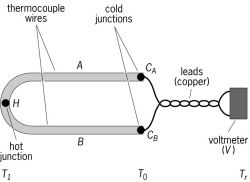
\includegraphics[width=0.5\linewidth]{thermocouple.jpg}
    \caption{Basic circuit of a thermocouple}%
    \label{fig:}
\end{figure}
\begin{itemize}
    %\item Thermoelectric devices create voltage from temperature differences.

    %\item Thermocouples are used in temperature measurement equipment and in various automatic control and monitoring systems. A thermoelectric thermometer is produced by combining a thermocouple with an electrical measurement instrument, such as a millivoltmeter or potentiometer. The measurement instrument is connected to the ends of the thermoelectrodes or to a break in one of the electrodes. When making a temperature measurement, one of the junctions must be maintained at a reference temperature, usually 273°K.


    \item This temperature measuring instrument consisting of two wires of different
metals joined at each end.
\item One junction is placed where the temperature is to be measured, and the other is kept at a constant lower (reference) temperature.
\item A measuring instrument is connected in the electrical
circuit.
\item The temperature difference causes the development of an electromotive force that is approximately proportional to the difference between the temperatures of the two junctions.
\item Temperature can be read from standard tables, or the instrument can be calibrated to display temperature directly
\end{itemize}
\subsection{Uses}
\begin{itemize}
\item It is used for obtaining temperatures internally or on the surface of body.
\item The unit is equipped with a variety of probes for obtaining
temperatures.
\item The thermionic thermometer offers greater accuracy than clinical mercury thermometer.
\item It can be located up to 1,000 ft from the unit and registers the temperature in about 5 seconds.

\end{itemize}

\section{Patient monitor}
%\begin{itemize}
    %\item
A patient monitor is an electronic medical device that consists of one of more monitoring sensors, a processing component(s), and a screen display (also called a "monitor") that provide and record for medical professionals a patient's medical vital signs (body temperature, blood pressure, pulse rate and respiratory rate) or measurements of the activity of various body organs such as ECG monitors, anesthesia monitors, or EKG monitors.


%\end{itemize}
\subsection{Working}
\begin{itemize}
    \item The transducer changes the physiologic information into
electric energy, which is then passed through electronic circuits.
\item These
circuits amplify the electrical impulses and may transform them into
mechanical energy in the form of a moving stylus that records the
patient’s pulse, temperatures, respirations and blood pressure on a
graph.
\item
Other monitors are equipped to flash lights or ring bells if patient
is exceeding certain physiological limits that have been programmed
into the circuits
\end{itemize}
\subsection{Uses}
\begin{itemize}
%\item Medical professionals and healthcare providers routinely monitor four main vital signs: body temperature, pulse rate, respiratory rate and blood pressure. In the medical practice of cardiology, the measurement and recording of the electrical activity of the heart over a period of time (known as ECG / EKG or electrocardiography) is also fundamental to patient care.

\item Multi-parameter patient monitors support the conduct of patient care in doctors’ offices, outpatient facilities, hospital operating rooms, hospital critical care facilities, and during EMS and non-emergency ambulance transport.
\item There may also be a need for bedside measurement of vital signs in low-acuity post-anesthetic care and during sleep studies.

%\item Particular vital signs may be the most important to monitor in varying medical situations. For example, the measurement of SpO2 (“saturation of peripheral oxygen”) is needed during surgery and in the recovery room to ensure proper patient care.

\item Multi-parameter patient monitors provide the composite view required, at a glance. Many include configurable vital signs settings and both audio and visual comprehensive alarms.

    %Various sizes exist, with variable numbers of parameters monitored. Portability and multi-use capabilities offer high cost-performance ratios by negating the need for multiple types of monitors. This vital equipment provides care teams more of the information they need while at the patient’s side.
\end{itemize}
\begin{figure}
    \centering
    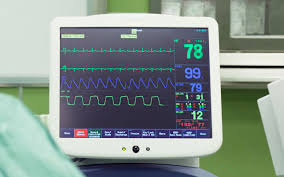
\includegraphics[width=0.6\linewidth]{patientmonitor.jpeg}
    \caption{A patient monitor}%
    \label{fig:}
\end{figure}
\section{Cathode Ray Oscilloscope}
\begin{itemize}

\item The basic operation on which the instrument function is a stream of electrons that are liberated from a hot filament or cathode.
\item The electron stream then passed through an anode at a high potential and strikes 	a fluorescent screen at the end of the tube.
\item Whenever an electron strikes a fluorescent screen a spot of light appears.
%Use
\item The electron stream is deflected from pursuing a straight path by an amplified current that is received from the part of the body under study.
\item This action current is connected to a pair of horizontal plates that deflect the electrons vertically and vice versa.
\item The picture produced on the screen is a pattern of these deflections as the beam
sweeps horizontally across the screen.

\item The light pattern formed may
be studied immediately or a photograph may be recorded for future
study.

\end{itemize}
\begin{figure}
    \centering
    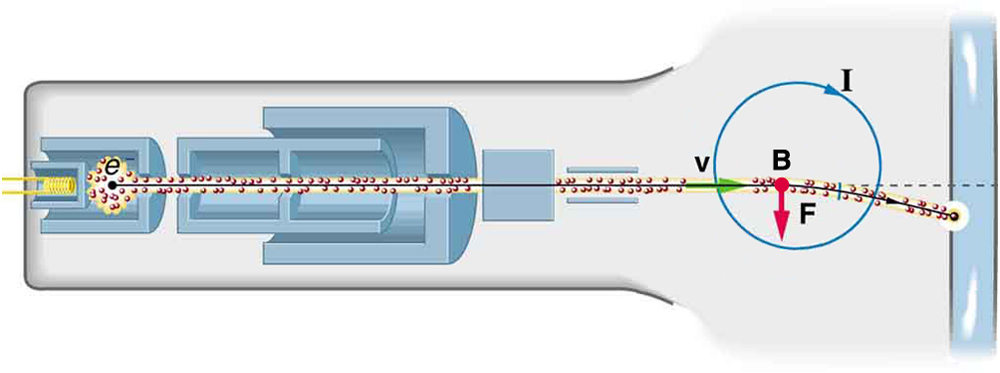
\includegraphics[width=0.8\linewidth]{crtube.jpeg}
    \caption{The cathode ray tube (CRT) is so named because rays of electrons originate at the cathode in the electron gun. Magnetic coils are used to steer the beam in many CRTs. In this case, the beam is moved down. Another pair of horizontal coils would steer the beam horizontally.}
    \label{fig:cro}
\end{figure}
\section{Electron microscope}
\begin{itemize}

    \item It depends upon the properties of electron for its operation.
The ordinary microscopes cannot be used to view objects less
than 0.000039 cm in diameter which is the same in magnitude
as the shortest wavelength of visible light.
\item Electrons possess a wave property similar to that of light waves.
The wavelength emitted depends upon the voltage with which the
electrons are accelerated.

\item Under certain conditions the wavelength
may be 0.05  \AA  . This is so much shorter than the shorter wavelength
of visible lights (3,900   \AA  ) that such minute objects as bateriophage
particles have been seen with the aid of the electron microscope.

\item The electron beam is provided by an electron gun. It contains an
anode with a small opening to allow the electrons to pass through.
The anode is grounded while the filament is at a negative voltage
of 50,000 or more.

\item There is also a doughnut-shaped coil of wire
that acts on electrons like a convex lens, bending them on the
object.

\item  The electrons beam is altered by the material by being
stopped, retarded or scattered.

\item The electrons beam is then passed through another electron lens that corresponds to the objective of optical microscope.
A third lens magnifies the image that is then focused on a fluorescent screen where it may be seen or
photographed.

\item Difference between electron microscope and ordinary microscope:
 Stream of fast moving electrons instead of light rays.
 Coils of wire in place of lenses.
 A fluorescent screen or photographic plate instead of eyepiece.

\end{itemize}

\begin{figure}
    \centering
    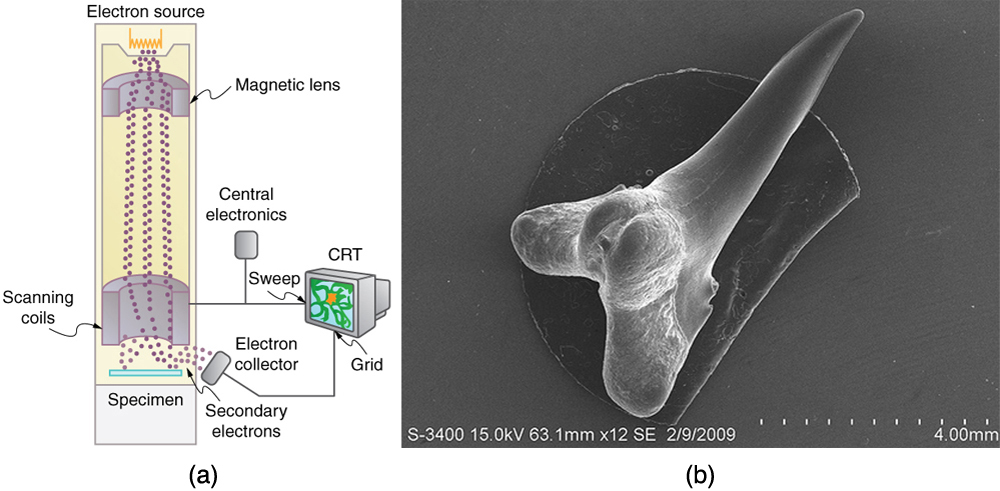
\includegraphics[width=\linewidth]{sem.jpeg}
    \caption{Schematic of a scanning electron microscope (SEM) (a) used to observe small details, such as those seen in this image of a tooth of a Himipristis, a type of shark (b).}%
    \label{fig:sem}
\end{figure}
\section{Diathermy}
\begin{itemize}
    \item The passage of any electric current through tissues will cause
heating. To obtain a significant amount of heat with ordinary low
frequency currents it would be necessary to use large amount of
current that the tissue would be destroyed.

\item High frequency current
however may be passed through tissues for a heating effect without
causing damage.

\item Diathermy is a means of producing heat in tissues
of the body by use of high frequency electric currents.
\end{itemize}
\subsection{Uses}
\begin{itemize}
\item Diathermy has been reported effective in traumatic and
inflammatory conditions of the skeleton for relief of bronchitis
and pain of pleurisy.
\item Ultra-high frequency diathermy may be used for inducing fever.
This reaction known as electropyrexia is of value in the treatment
of general paresis.
\end{itemize}


%\begin{thebibliography}{8}
    %\bibitem{Free} Thermocouples  \url{https://encyclopedia2.thefreedictionary.com/}
%\end{thebibliography}
\end{document}
